% Options for packages loaded elsewhere
% Options for packages loaded elsewhere
\PassOptionsToPackage{unicode}{hyperref}
\PassOptionsToPackage{hyphens}{url}
\PassOptionsToPackage{dvipsnames,svgnames,x11names}{xcolor}
%
\documentclass[
  11pt,
  a4paper,
]{report}
\usepackage{xcolor}
\usepackage[top=25mm,left=25mm,right=25mm,bottom=25mm]{geometry}
\usepackage{amsmath,amssymb}
\setcounter{secnumdepth}{3}
\usepackage{iftex}
\ifPDFTeX
  \usepackage[T1]{fontenc}
  \usepackage[utf8]{inputenc}
  \usepackage{textcomp} % provide euro and other symbols
\else % if luatex or xetex
  \usepackage{unicode-math} % this also loads fontspec
  \defaultfontfeatures{Scale=MatchLowercase}
  \defaultfontfeatures[\rmfamily]{Ligatures=TeX,Scale=1}
\fi
\usepackage{lmodern}
\ifPDFTeX\else
  % xetex/luatex font selection
  \setmainfont[]{Source Sans 3}
  \setsansfont[]{Source Sans 3}
  \setmonofont[Scale=0.8125]{Monaspace Neon}
\fi
% Use upquote if available, for straight quotes in verbatim environments
\IfFileExists{upquote.sty}{\usepackage{upquote}}{}
\IfFileExists{microtype.sty}{% use microtype if available
  \usepackage[]{microtype}
  \UseMicrotypeSet[protrusion]{basicmath} % disable protrusion for tt fonts
}{}
\usepackage{setspace}
\makeatletter
\@ifundefined{KOMAClassName}{% if non-KOMA class
  \IfFileExists{parskip.sty}{%
    \usepackage{parskip}
  }{% else
    \setlength{\parindent}{0pt}
    \setlength{\parskip}{6pt plus 2pt minus 1pt}}
}{% if KOMA class
  \KOMAoptions{parskip=half}}
\makeatother
% Make \paragraph and \subparagraph free-standing
\makeatletter
\ifx\paragraph\undefined\else
  \let\oldparagraph\paragraph
  \renewcommand{\paragraph}{
    \@ifstar
      \xxxParagraphStar
      \xxxParagraphNoStar
  }
  \newcommand{\xxxParagraphStar}[1]{\oldparagraph*{#1}\mbox{}}
  \newcommand{\xxxParagraphNoStar}[1]{\oldparagraph{#1}\mbox{}}
\fi
\ifx\subparagraph\undefined\else
  \let\oldsubparagraph\subparagraph
  \renewcommand{\subparagraph}{
    \@ifstar
      \xxxSubParagraphStar
      \xxxSubParagraphNoStar
  }
  \newcommand{\xxxSubParagraphStar}[1]{\oldsubparagraph*{#1}\mbox{}}
  \newcommand{\xxxSubParagraphNoStar}[1]{\oldsubparagraph{#1}\mbox{}}
\fi
\makeatother


\usepackage{longtable,booktabs,array}
\newcounter{none} % for unnumbered tables
\usepackage{calc} % for calculating minipage widths
% Correct order of tables after \paragraph or \subparagraph
\usepackage{etoolbox}
\makeatletter
\patchcmd\longtable{\par}{\if@noskipsec\mbox{}\fi\par}{}{}
\makeatother
% Allow footnotes in longtable head/foot
\IfFileExists{footnotehyper.sty}{\usepackage{footnotehyper}}{\usepackage{footnote}}
\makesavenoteenv{longtable}
\usepackage{graphicx}
\makeatletter
\newsavebox\pandoc@box
\newcommand*\pandocbounded[1]{% scales image to fit in text height/width
  \sbox\pandoc@box{#1}%
  \Gscale@div\@tempa{\textheight}{\dimexpr\ht\pandoc@box+\dp\pandoc@box\relax}%
  \Gscale@div\@tempb{\linewidth}{\wd\pandoc@box}%
  \ifdim\@tempb\p@<\@tempa\p@\let\@tempa\@tempb\fi% select the smaller of both
  \ifdim\@tempa\p@<\p@\scalebox{\@tempa}{\usebox\pandoc@box}%
  \else\usebox{\pandoc@box}%
  \fi%
}
% Set default figure placement to htbp
\def\fps@figure{htbp}
\makeatother


% definitions for citeproc citations
\NewDocumentCommand\citeproctext{}{}
\NewDocumentCommand\citeproc{mm}{%
  \begingroup\def\citeproctext{#2}\cite{#1}\endgroup}
\makeatletter
 % allow citations to break across lines
 \let\@cite@ofmt\@firstofone
 % avoid brackets around text for \cite:
 \def\@biblabel#1{}
 \def\@cite#1#2{{#1\if@tempswa , #2\fi}}
\makeatother
\newlength{\cslhangindent}
\setlength{\cslhangindent}{1.5em}
\newlength{\csllabelwidth}
\setlength{\csllabelwidth}{3em}
\newenvironment{CSLReferences}[2] % #1 hanging-indent, #2 entry-spacing
 {\begin{list}{}{%
  \setlength{\itemindent}{0pt}
  \setlength{\leftmargin}{0pt}
  \setlength{\parsep}{0pt}
  % turn on hanging indent if param 1 is 1
  \ifodd #1
   \setlength{\leftmargin}{\cslhangindent}
   \setlength{\itemindent}{-1\cslhangindent}
  \fi
  % set entry spacing
  \setlength{\itemsep}{#2\baselineskip}}}
 {\end{list}}
\usepackage{calc}
\newcommand{\CSLBlock}[1]{\hfill\break\parbox[t]{\linewidth}{\strut\ignorespaces#1\strut}}
\newcommand{\CSLLeftMargin}[1]{\parbox[t]{\csllabelwidth}{\strut#1\strut}}
\newcommand{\CSLRightInline}[1]{\parbox[t]{\linewidth - \csllabelwidth}{\strut#1\strut}}
\newcommand{\CSLIndent}[1]{\hspace{\cslhangindent}#1}



\setlength{\emergencystretch}{3em} % prevent overfull lines

\providecommand{\tightlist}{%
  \setlength{\itemsep}{0pt}\setlength{\parskip}{0pt}}



 


\usepackage{lipsum}
\usepackage{fancyhdr}
\usepackage{xcolor}
\definecolor{draftred}{RGB}{180,0,0}
\pagestyle{fancy}
\fancyhead[L]{ {\footnotesize {Report: Vocabulary growth in children with Down syndrome}}}
\fancyhead[R]{\textbf{\textcolor{draftred}{DRAFT}}}
\fancyfoot[L]{ {\ttfamily\footnotesize 2026-07-01} | {\ttfamily\footnotesize 0.1.0} | {\ttfamily\footnotesize "dev"} }%
\fancyfoot[C]{}
\fancyfoot[R]{\textbf{\thepage}}  
\renewcommand{\chaptername}{Section}

% --- make chapter-opening pages use the same header/footer ---
\fancypagestyle{plain}{%
  \fancyhf{}%
  \fancyhead[L]{ {\footnotesize {Report: Vocabulary growth in children with Down syndrome}}}%
    \fancyhead[R]{\textbf{\textcolor{draftred}{DRAFT}}}%
    \fancyfoot[L]{ {\ttfamily\footnotesize 2026-07-01} | {\ttfamily\footnotesize 0.1.0} | {\ttfamily\footnotesize "dev"} }%
  \fancyfoot[R]{\textbf{\thepage}}%
  \renewcommand{\headrulewidth}{0.4pt}%
  \renewcommand{\footrulewidth}{0pt}%
}
\makeatletter
\@ifpackageloaded{tcolorbox}{}{\usepackage[skins,breakable]{tcolorbox}}
\@ifpackageloaded{fontawesome5}{}{\usepackage{fontawesome5}}
\definecolor{quarto-callout-color}{HTML}{909090}
\definecolor{quarto-callout-note-color}{HTML}{0758E5}
\definecolor{quarto-callout-important-color}{HTML}{CC1914}
\definecolor{quarto-callout-warning-color}{HTML}{EB9113}
\definecolor{quarto-callout-tip-color}{HTML}{00A047}
\definecolor{quarto-callout-caution-color}{HTML}{FC5300}
\definecolor{quarto-callout-color-frame}{HTML}{acacac}
\definecolor{quarto-callout-note-color-frame}{HTML}{4582ec}
\definecolor{quarto-callout-important-color-frame}{HTML}{d9534f}
\definecolor{quarto-callout-warning-color-frame}{HTML}{f0ad4e}
\definecolor{quarto-callout-tip-color-frame}{HTML}{02b875}
\definecolor{quarto-callout-caution-color-frame}{HTML}{fd7e14}
\makeatother
\makeatletter
\@ifpackageloaded{bookmark}{}{\usepackage{bookmark}}
\makeatother
\makeatletter
\@ifpackageloaded{caption}{}{\usepackage{caption}}
\AtBeginDocument{%
\ifdefined\contentsname
  \renewcommand*\contentsname{Table of contents}
\else
  \newcommand\contentsname{Table of contents}
\fi
\ifdefined\listfigurename
  \renewcommand*\listfigurename{List of Figures}
\else
  \newcommand\listfigurename{List of Figures}
\fi
\ifdefined\listtablename
  \renewcommand*\listtablename{List of Tables}
\else
  \newcommand\listtablename{List of Tables}
\fi
\ifdefined\figurename
  \renewcommand*\figurename{Figure}
\else
  \newcommand\figurename{Figure}
\fi
\ifdefined\tablename
  \renewcommand*\tablename{Table}
\else
  \newcommand\tablename{Table}
\fi
}
\@ifpackageloaded{float}{}{\usepackage{float}}
\floatstyle{ruled}
\@ifundefined{c@chapter}{\newfloat{codelisting}{h}{lop}}{\newfloat{codelisting}{h}{lop}[chapter]}
\floatname{codelisting}{Listing}
\newcommand*\listoflistings{\listof{codelisting}{List of Listings}}
\makeatother
\makeatletter
\makeatother
\makeatletter
\@ifpackageloaded{caption}{}{\usepackage{caption}}
\@ifpackageloaded{subcaption}{}{\usepackage{subcaption}}
\makeatother
\usepackage{bookmark}
\IfFileExists{xurl.sty}{\usepackage{xurl}}{} % add URL line breaks if available
\urlstyle{same}
\hypersetup{
  pdftitle={Vocabulary growth in children with Down syndrome},
  pdfauthor={Frank Buckley; Sue Buckley},
  colorlinks=true,
  linkcolor={blue},
  filecolor={Maroon},
  citecolor={Blue},
  urlcolor={Blue},
  pdfcreator={LaTeX via pandoc}}


\title{Vocabulary growth in children with Down syndrome}
\author{Frank Buckley \and Sue Buckley}
\date{2026-07-01}
\begin{document}
\maketitle

\renewcommand*\contentsname{Table of contents}
{
\setcounter{tocdepth}{2}
\tableofcontents
}

\setstretch{1.25}
\bookmarksetup{startatroot}

\chapter*{Preface}\label{preface}
\addcontentsline{toc}{chapter}{Preface}

\markboth{Preface}{Preface}

This technical report describes an exploratory study of vocabulary
development in children with Down syndrome that aims to characterise
observed trajectories of word learning, spoken and gestured production,
and relationships between words understood and produced. The primary
goal of the study is to provide interpretable statistics that can
accurately inform expectations, intervention and teaching practice.

The study develops statistical models consistent with empirical models
of vocabulary learning. We evaluate and fit these models using Bayesian
inference to estimate full probability distributions for parameters of
interest (\citeproc{ref-gelmanBayesianDataAnalysis2013}{Gelman et al.,
2013}; \citeproc{ref-gelmanRegressionOtherStories2020}{Gelman, Hill, et
al., 2020};
\citeproc{ref-mcelreathStatisticalRethinkingBayesian2020}{McElreath,
2020};
\citeproc{ref-wagenmakersBayesianInferencePsychology2018}{Wagenmakers et
al., 2018}), using an iterative workflow
(\citeproc{ref-gelmanBayesianWorkflow2020}{Gelman, Vehtari, et al.,
2020}). This results in models that reflect empirical constraints and
available evidence, and that provide more realistic and more precise
estimates than are possible if we build models that ignore existing
knowledge (\citeproc{ref-gillBayesianSocialScience2024}{Gill \& Bao,
2024};
\citeproc{ref-mcelreathStatisticalRethinkingBayesian2020}{McElreath,
2020}).

There are further benefits to this approach. Developing explicit models
helps us to communicate more clearly -- to be unambiguous about our
empirical and statistical assumptions
(\citeproc{ref-farrellComputationalModelingCognition2018}{Farrell \&
Lewandowsky, 2018}). Building computational and statistical models also
allows us to test and validate these assumptions
(\citeproc{ref-farrellComputationalModelingCognition2018}{Farrell \&
Lewandowsky, 2018};
\citeproc{ref-mcelreathStatisticalRethinkingBayesian2020}{McElreath,
2020}).

To contribute to continuing progress, we should describe our methods and
explain our results in sufficient detail for others to replicate our
findings. That description is incomplete without source code for all
models that can be run using freely available software
(\citeproc{ref-farrellComputationalModelingCognition2018}{Farrell \&
Lewandowsky, 2018};
\citeproc{ref-mcelreathStatisticalRethinkingBayesian2020}{McElreath,
2020}). This is the purpose of this technical report and the
accompanying repository
(\url{https://github.com/dseinternational/vocabulary-growth}).

We have tried to write this report for a broad possible audience, while
aiming to meet recommended reporting practices
(\citeproc{ref-kruschkeBayesianAnalysisReporting2021}{Kruschke, 2021};
\citeproc{ref-schubertImprovingStatisticalReporting2025}{Schubert et
al., 2025}). It therefore may not suit everyone. We cannot avoid
statistical and computational details, but we try to explain as much as
we can for readers for whom these may not be familiar. For readers who
would prefer a shorter overview of our methods and our findings, a
summary report is also available {[}TODO: link{]}.

Scientific and statistical texts include many terms that are intended to
have precise meanings in specific contexts but are not always used to
mean precisely the same things by all authors in all disciplines. We
therefore include a glossary to be precise about our intended meanings
for important terms used in this report.

Discovery and learning are ongoing processes. One of the reasons for
adopting the methods we have used in this study is to explore models
that may have wider application and that may encourage further research.
Models that accommodate nonlinear relationships between variables,
considerable variability within the population, and that can reflect
existing evidence are (we think) likely to help inform better
statistical analyses in many areas of Down syndrome research.

To that end, this study is not fixed in time. As new data becomes
available, we anticipate updating our estimates and evolving our models.
We will version the study as in software development -- tagging releases
in the study repository whenever we publish updated analyses. We hope
that ``version 1.0'' is helpful and of interest to families,
practitioners and researchers alike, and welcome feedback,
collaboration, and contributions to future iterations.

\bookmarksetup{startatroot}

\chapter*{Acknowledgements}\label{acknowledgements}
\addcontentsline{toc}{chapter}{Acknowledgements}

\markboth{Acknowledgements}{Acknowledgements}

{[}TODO{]}

\bookmarksetup{startatroot}

\chapter*{Summary}\label{summary}
\addcontentsline{toc}{chapter}{Summary}

\markboth{Summary}{Summary}

{[}TODO{]}

\bookmarksetup{startatroot}

\chapter*{Glossary}\label{glossary}
\addcontentsline{toc}{chapter}{Glossary}

\markboth{Glossary}{Glossary}

TODO

\part{Background and aims}

\chapter{Introduction}\label{introduction}

\emph{All children with Down syndrome experience delays in language
development. By quantifying typical trajectories of vocabulary
development we can offer families and practitioners insights into
expected ranges and rates of progress. These can help to inform teaching
goals and methods, and to identify children experiencing more complex or
challenging difficulties. This study aims to provide accurate estimates
of typical trajectories of word learning and distributions of expected
spoken and understood word counts at six monthly intervals for children
with Down syndrome aged 12 months to 8 years. Here, we discuss the
rationale for the study, our goals, and our empirical and statistical
modelling approaches.}

\hfill\break

Children with Down syndrome experience difficulties learning language
(\citeproc{ref-abbedutoLanguageDevelopmentSyndrome2020}{Abbeduto et al.,
2020}; \citeproc{ref-naessLanguageVerbalShortterm2011}{Næss et al.,
2011}) and this adversely impacts many aspect of their lives. They learn
the meanings of words and learn to say words more slowly than most other
children (\citeproc{ref-naessDifferencesSimilaritiesPredictors2021}{Næss
et al., 2021}). Learning vocabulary is a foundational skill: it is
important for learning broader language skills, including grammar, and
for learning to read (\citeproc{ref-hulmeGrowthReadingSkills2012}{Hulme
et al., 2012}; \citeproc{ref-naessReadingSkillsChildren2012}{Næss et
al., 2012}).

Parents and practitioners working with people with Down syndrome report
that past research has not focussed enough on practical issues that
might make meaningful differences to their lives
(\citeproc{ref-cristescuShapeResearchChange2024}{Cristescu et al.,
2024}). This has led to calls for researchers to makes it easier for
families and educators to access evidence-based information to inform
decisions related to real life issues
(\citeproc{ref-cristescuShapeResearchChange2024}{Cristescu et al.,
2024}).

In our experience, families and educators are often interested in
information about vocabulary development in children with Down syndrome.
Common requests for information include the range of words understood or
spoken at different ages, rates of word learning, and the range of ages
at which a minimum number of words may be learned. Answers to questions
about vocabulary development are of relevance to everyday teaching
practice and early intervention. They may alleviate unwarranted concerns
about slow progress and help to identify children experiencing
additional or more complex difficulties. They can also inform teaching
recommendations -- for example, by estimating the range of ages within
which most children are expected to attain specific skills.

This study therefore aims to describe the development of vocabulary
knowledge in children with Down syndrome with a focus on interpretable
statistics that can inform teaching and support.

\section{Vocabulary learning for children with Down
syndrome}\label{vocabulary-learning-for-children-with-down-syndrome}

Children with Down syndrome generally learn vocabulary more slowly than
typically developing children
(\citeproc{ref-abbedutoLanguageDevelopmentSyndrome2020}{Abbeduto et al.,
2020}). They generally say fewer words than they understand and there
are considerable differences between individuals that increase over time
(\citeproc{ref-berglundParentalReportsSpoken2001}{Berglund et al.,
2001}; \citeproc{ref-deckersPredictorsReceptiveExpressive2019}{Deckers
et al., 2019};
\citeproc{ref-galeoteAcquisitionProductiveVocabulary2008}{Galeote et
al., 2008};
\citeproc{ref-kaat-vandenosExpressiveVocabularyDevelopment2017}{Kaat-van
Den Os et al., 2017};
\citeproc{ref-oliverLanguageDevelopmentChildren1994}{Oliver \& Buckley,
1994}; \citeproc{ref-zampiniVocabularyDevelopmentChildren2013}{Zampini
\& D'Odorico, 2013}).

Many children with Down syndrome produce their first spoken word later
than typically developing infants, with some not saying their first
words until after 24 months of age, though there is wide variability and
some begin at around the same time. In comparison, 80\% of typically
developing children say 2 or more words by around 12 months and 90\% say
7 or more words by around 18 months
(\citeproc{ref-frankWordbankOpenRepository2017}{Frank et al., 2017}).
While some children with Down syndrome learn the first 10 spoken words
between the ages of 19 and 38 months
(\citeproc{ref-oliverLanguageDevelopmentChildren1994}{Oliver \& Buckley,
1994}), over 80\% of typically developing children reach this stage by
17 months (\citeproc{ref-frankWordbankOpenRepository2017}{Frank et al.,
2017}).

At a basic level, general cognitive delays may imply that children with
Down syndrome need more exposures to a word to link it reliably to its
meaning. Additionally, many children with Down syndrome experience
recurrent or persistent hearing loss, especially in early childhood,
which affects discrimination of speech sounds and makes it harder to
distinguish similar‑sounding words (for example, ``cat/hat/mat''). Even
mild hearing loss may impede building accurate sound--meaning links.
Anatomical differences (including a smaller oral cavity and larger
tongue) may make articulation more difficult. Delays in babbling and
moving from babble to clear word production may lead children with Down
syndrome to rely on gestures for longer before attempting spoken words.
Difficulties storing accurate sound patterns may affect both word
learning and clear pronunciation. Verbal short-term memory is typically
impaired relative to visuospatial short-term memory in Down syndrome.
This may make it more difficult to hold new word forms in mind, repeat
unfamiliar words or nonwords, and process longer utterances.

\subsection{Relative disadvantage in expressive vocabulary
development}\label{relative-disadvantage-in-expressive-vocabulary-development}

The extent to which expressive vocabulary lags behind receptive
vocabulary disproportionately compared to typically developing children
is not clear, and may depend on how vocabulary is measured, whether
gestures are included, the age of the children and how groups are
compared
(\citeproc{ref-abbedutoLanguageDevelopmentSyndrome2020}{Abbeduto et al.,
2020};
\citeproc{ref-martingklusekjestigarribiabjLanguageCharacteristicsIndividuals2009}{Martin,
2009}). One recent study involving 27 children with Down syndrome aged
12 to 39 months observed a pattern of spoken words relative to words
understood that was similar to typically developing children, but
dissimilar to children with Williams syndrome and children with fragile
X syndrome
(\citeproc{ref-dsouzaExplainingComprehensionProduction2026}{D'Souza et
al., 2026}). However, it remains unclear whether this similarity is
observed across larger samples, nor if it persists as more vocabulary is
learned.

{[}\textbf{TODO}: complete{]}

\subsection{Rates of word learning}\label{rates-of-word-learning}

Word learning accelerates rapidly for many typically developing children
between the ages of 18 and 24 months. It is unclear whether children
with Down syndrome experience a similar acceleration, with some studies
observing an acceleration among some children and not others, and any
acceleration occurring later than for typically developing children
though maybe at a similar mental age
(\citeproc{ref-abbedutoLanguageDevelopmentSyndrome2020}{Abbeduto et al.,
2020}; \citeproc{ref-berglundParentalReportsSpoken2001}{Berglund et al.,
2001}; \citeproc{ref-oliverLanguageDevelopmentChildren1994}{Oliver \&
Buckley, 1994};
\citeproc{ref-zampiniVocabularyDevelopmentChildren2013}{Zampini \&
D'Odorico, 2013}).

{[}\textbf{TODO}: complete{]}

\subsection{Use of gestures and signs}\label{use-of-gestures-and-signs}

{[}\textbf{TODO}: complete{]}

\section{Study aims and approach}\label{study-aims-and-approach}

{[}\textbf{TODO}{]}

\section{Modelling and inference}\label{modelling-and-inference}

Statistical modelling and inference provide methods for defining
mathematical models and evaluating them against data to obtain
evidence-based estimates of the parameters of interest
(\citeproc{ref-chanStatisticalModelingComputation2025}{Chan \& Kroese,
2025}; \citeproc{ref-coxPrinciplesStatisticalInference2006}{Cox, 2006};
\citeproc{ref-farrellComputationalModelingCognition2018}{Farrell \&
Lewandowsky, 2018}; \citeproc{ref-gelmanBayesianDataAnalysis2013}{Gelman
et al., 2013}; \citeproc{ref-gelmanRegressionOtherStories2020}{Gelman,
Hill, et al., 2020};
\citeproc{ref-mcelreathStatisticalRethinkingBayesian2020}{McElreath,
2020}; \citeproc{ref-spanosProbabilityTheoryStatistical2019}{Spanos,
2019};
\citeproc{ref-wakefieldBayesianFrequentistRegression2013}{Wakefield,
2013}). They are central to evaluating scientific theories and
interpreting data, and can express what a theory means more precisely
than words alone
(\citeproc{ref-farrellComputationalModelingCognition2018}{Farrell \&
Lewandowsky, 2018, Chapter 1}).

A statistical model is a set of assumptions describing a process that
could generate the data, relating the parameters of interest to what we
observe. Because a model can also generate synthetic datasets consistent
with those assumptions, we can simulate from it to check that it behaves
as intended
(\citeproc{ref-farrellComputationalModelingCognition2018}{Farrell \&
Lewandowsky, 2018};
\citeproc{ref-mcelreathStatisticalRethinkingBayesian2020}{McElreath,
2020}). Statistical inference then uses the model and the observed data
to estimate its unknown parameters, test specific claims, predict future
observations, and quantify how uncertain those conclusions are.

\subsection{Statistical models}\label{statistical-models}

Statistical models do not by themselves explain how the world works,
though they can evaluate the predictions of models that do. A regression
model reveals statistical relationships between predictors and outcomes,
but those relationships acquire their real-world relevance only within
an \emph{empirical model} --- an account of the real-world phenomenon
that informs which statistical and process models can test
it.\footnote{For a perspective on empirical modelling as a process for
  ``learning from data'' using statistical models, see Spanos
  (\citeproc{ref-spanosProbabilityTheoryStatistical2019}{2019, Chapter
  1}). For further discussion of empirical, process-based and
  statistical models, see Van Oijen
  (\citeproc{ref-vanoijenBayesianCompendium2024}{2024, Chapter 1}). For
  further discussion of computational process models, see Farrell and
  Lewandowsky
  (\citeproc{ref-farrellComputationalModelingCognition2018}{2018,
  Chapter 1}).}

For example, we might explain word learning by proposing that children
learn word meanings by hearing words spoken and recognising what they
refer to. That explanation predicts that, as children have more
opportunities to hear words, they will understand more of them over time
--- and we can build statistical models to test whether the observed
data match that prediction (rising counts of words understood with age).

The mapping between the two runs both ways: one empirical model admits
many statistical models, and one statistical model is consistent with
many empirical models. So even when a statistical model fits the
observed data well, we cannot be certain its motivating explanation is
`the right one' --- another, equally credible, explanation may fit just
as well:

\begin{quote}
``Many models correspond to the same hypothesis, and many hypotheses
correspond to a single model. This makes strict falsification
impossible.''
(\citeproc{ref-mcelreathStatisticalRethinkingBayesian2020}{McElreath,
2020, p. 4})
\end{quote}

Developing and evaluating models is therefore continual and iterative
(\citeproc{ref-gelmanBayesianWorkflow2020}{Gelman, Vehtari, et al.,
2020}): a competing model may explain the data better, and new
observations refine existing models, revise theories and motivate new
ones --- the workflow this report follows throughout
(\textbf{?@sec-lineage-ds}).

\subsection{Inference}\label{inference}

There are different approaches to statistical inference, differing in
their philosophical and mathematical foundations and in the conclusions
they license (\citeproc{ref-gelmanBayesianDataAnalysis2013}{Gelman et
al., 2013};
\citeproc{ref-mcelreathStatisticalRethinkingBayesian2020}{McElreath,
2020}; \citeproc{ref-spanosProbabilityTheoryStatistical2019}{Spanos,
2019};
\citeproc{ref-wakefieldBayesianFrequentistRegression2013}{Wakefield,
2013}). Bayesian methods remain uncommon in developmental Down syndrome
research, but for the questions this study addresses they offer four
concrete advantages, set out below: probability statements that mean
what families take them to mean; uncertainty expressed as full
distributions; a principled way to bring existing knowledge to bear; and
direct predictions about individual children.

\subsubsection{Probability as
uncertainty}\label{probability-as-uncertainty}

Bayesian inference treats probability as a measure of uncertainty about
unknown quantities -- ``relative, in part to this ignorance, in part to
our knowledge''
(\citeproc{ref-laplaceEssaiPhilosophiqueProbabilites1814}{LaPlace,
1814}) -- so that a number near one marks an event we consider very
likely and one near zero an event we consider very unlikely
(\citeproc{ref-gillBayesianSocialScience2024}{Gill \& Bao, 2024}). On a
partly cloudy day, ``a 50\% chance of rain this afternoon'' means that,
given what we currently know, rain and no rain seem about equally
plausible.

A different approach -- frequentist inference, long dominant in science
and still standard in this field -- defines probability as the long-run
relative frequency of an event under repeated, comparable trials
(\citeproc{ref-spanosProbabilityTheoryStatistical2019}{Spanos, 2019};
\citeproc{ref-wakefieldBayesianFrequentistRegression2013}{Wakefield,
2013}). The same forecast becomes a calibration claim about a
\emph{method}: across many past occasions when it said ``50\%'', it
rained about half the time, so estimates are judged by long-run
properties such as unbiasedness and interval coverage
(\citeproc{ref-gelmanRegressionOtherStories2020}{Gelman, Hill, et al.,
2020}). That framing suits settings such as industrial quality control,
where repetition under fixed conditions is real and controlling error
rates is the goal. Much developmental research is not like that: small
samples, many interacting influences on several outcomes, and wide
variation between children
(\citeproc{ref-wagenmakersBayesianInferencePsychology2018}{Wagenmakers
et al., 2018}). For this study, the Bayesian reading of probability lets
us make statements about our estimates that a broad readership will
interpret correctly.

\subsubsection{Estimates as
distributions}\label{estimates-as-distributions}

Bayesian inference begins with a prior distribution -- what we consider
plausible before seeing the data -- and uses Bayes' theorem to update it
into a posterior distribution that combines prior and data, with
uncertainty built in and shown by how peaked or flat the posterior is
(\citeproc{ref-gillBayesianSocialScience2024}{Gill \& Bao, 2024}).

Figure~\ref{fig-bayes-update-20} illustrates this. For a yes/no outcome
we begin with a weakly informative prior centred on \(p = 0.5\) (blue),
expecting all-yes or all-no to be less likely than intermediate values.
We then observe 20 simulated outcomes, 11 of them ``yes'' (green), and
apply Bayes' theorem to obtain the posterior (orange). With only 20
observations the sample is not centred on the true mean
(\(p_\text{obs} = 0.55\), \(p_\text{true} = 0.65\)); this weak prior
shifts and narrows the posterior only slightly, leaving it primarily
data-driven (\(p_\text{post} = 0.54\)).

\begin{figure}

\centering{

\pandocbounded{\includegraphics[keepaspectratio]{figures/bayes_update.png}}

}

\caption{\label{fig-bayes-update-20}\textbf{Bayesian updating}
(\(n = 20\)). Given a prior distribution (blue) and the observed data
(green), we use Bayes theorem to obtain the posterior distribution
(orange).}

\end{figure}%

Figure~\ref{fig-bayes-update-100} repeats this with the same prior and
true mean but 100 observations: the observed mean is closer to the truth
(\(p_\text{obs} = 0.61\)) and the posterior is more concentrated around
it (\(p_\text{post} = 0.61\)).

\begin{figure}

\centering{

\pandocbounded{\includegraphics[keepaspectratio]{figures/bayes_update_2.png}}

}

\caption{\label{fig-bayes-update-100}\textbf{Bayesian updating}
(\(n = 100\)). As Figure~\ref{fig-bayes-update-20}, but with 100
observations: the posterior distribution is now more concentrated around
the observed mean.}

\end{figure}%

Frequentist uncertainty is instead grounded in how an estimation
procedure behaves across repeated samples; a confidence interval is not
a probability statement about where the true value lies and does not
rank some values as more plausible than others
(\citeproc{ref-moreyFallacyPlacingConfidence2016}{Morey et al., 2016})
-- a distinction that is, unfortunately, often misinterpreted in
practice
(\citeproc{ref-hoekstraRobustMisinterpretationConfidence2014}{Hoekstra
et al., 2014}). A Bayesian posterior instead supports direct statements
such as: ``given our model and the data, the typical 36-month-old child
with Down syndrome learns about 5 new words per month, with a 90\%
probability that the typical rate lies between 2 and 7.'' These are the
statements families, practitioners and researchers tend to find useful
-- and, as McElreath observes, the ones ``scientists tend to project
onto statistical results'' in any case
(\citeproc{ref-mcelreathStatisticalRethinkingBayesian2020}{McElreath,
2020}). Bayesian inference is also logically coherent and well suited to
complex models (\citeproc{ref-bernardoBayesianStatistics2025}{Bernardo,
2025};
\citeproc{ref-wagenmakersBayesianFrequentistInference2008}{Wagenmakers
et al., 2008};
\citeproc{ref-wagenmakersBayesianInferencePsychology2018}{Wagenmakers et
al., 2018}).

\subsubsection{\texorpdfstring{From \emph{p}-values to posterior
probabilities}{From p-values to posterior probabilities}}\label{from-p-values-to-posterior-probabilities}

Readers used to frequentist reporting can map the familiar quantities
onto their Bayesian counterparts directly. A \textbf{credible interval}
is what a confidence interval is often mistaken for: a range that holds
the parameter with the stated probability, given the model and the data.
In place of a \emph{p}-value we report a \textbf{posterior tail
probability} -- the posterior mass on one side of a reference value,
such as the probability \(P(\psi > 1)\) that the sign--speech
association exceeds independence, or the probability that a trajectory
is rising. This reads as the probability of the claim itself, not the
probability of data at least as extreme were some null true.

Two consequences are worth stating plainly. First, a posterior can give
\textbf{evidence for a ``null''}: posterior mass concentrated near a
reference value is positive evidence that an effect is small, whereas a
non-significant \emph{p}-value can only \emph{fail to reject} one.
Second, a tail probability is \textbf{not a \emph{p}-value wearing a
different threshold}. For a roughly symmetric posterior the one-sided
tail probability (the ``probability of direction'', \(pd\)) and a
two-sided \emph{p}-value are related by \(p \approx 2\,(1 - pd)\), so
treating \(pd \ge 0.975\) as though it were ``significance at
\(p < 0.05\)'' merely reimports the significance grid this framing is
meant to retire. We therefore lead with the interval and the tail
probability, and where a verbal label is unavoidable we grade the
\emph{strength of the evidence} for a named claim on a transparent odds
scale (used for the sign--speech association in
\textbf{?@sec-findings-signing}) rather than against a fixed cut-off.

\subsubsection{Using existing knowledge}\label{using-existing-knowledge}

A prior encodes what is plausible about each parameter before the
current data are analysed. Priors can draw on previous research and the
experience of people with relevant expertise, or be weakly informative
-- ruling out implausible values while letting the data lead. A
well-grounded prior combined with the data yields estimates that are
more stable, and often more precise, than the data alone -- especially
valuable when datasets are small or noisy and a substantial evidence
base already exists.

The need to specify a prior is sometimes criticised as ``subjective''.
But every analysis rests on assumptions; the Bayesian ones are simply
explicit and open to scrutiny. A prior ``should be chosen, evaluated,
and revised just like all of the other components of the model''
(\citeproc{ref-mcelreathStatisticalRethinkingBayesian2020}{McElreath,
2020}), and we can test directly how sensitive our estimates are to it
(\citeproc{ref-gelmanBayesianWorkflow2020}{Gelman, Vehtari, et al.,
2020}). For this study, priors let us bring existing knowledge of
vocabulary development in children with Down syndrome to bear and
improve the accuracy of our estimates.

\subsubsection{Predictions for individual
children}\label{predictions-for-individual-children}

From the posterior we can also predict unobserved outcomes. Drawing
parameter values from the posterior and simulating a new observation for
each draw yields a \emph{posterior predictive distribution} that carries
both the randomness in the data and our uncertainty about the
parameters. This supports statements such as: ``given our model and the
data, there is a 90\% probability that a 36-month-old child with Down
syndrome understands between 0 and 142 words'' -- directly useful for
setting expectations about individual children.

\subsubsection{Computation}\label{computation}

Bayesian inference is centuries old
(\citeproc{ref-bayesLIIEssaySolving1763}{Bayes \& Price, 1763};
\citeproc{ref-LaplaceMemoireProbabilite}{LaPlace, 1774};
\citeproc{ref-laplaceTheorieAnalytiqueProbabilites1820}{LaPlace, 1820})
but became practical for all but the simplest models only with modern
sampling algorithms
(\citeproc{ref-hastingsMonteCarloSampling1970}{Hastings, 1970};
\citeproc{ref-hoffmanNoUTurnSamplerAdaptively2014}{Hoffman \& Gelman,
2014}; \citeproc{ref-metropolisEquationStateCalculations1953}{Metropolis
et al., 1953}), now packaged in accessible open-source tools such as
Stan and PyMC with interfaces to R and Python
(\citeproc{ref-abril-plaPyMCModernComprehensive2023}{Abril-Pla et al.,
2023}; \citeproc{ref-standevelopmentteamStanLanguageReference2026}{Stan
Development Team, 2026}). It is consequently now used across economics,
political science, ecology, biology, neuroscience, medicine, psychology
and education research (\citeproc{ref-bonBeingBayesian2020s2023}{Bon et
al., 2023}; \citeproc{ref-gillBayesianModelingInference2020}{Gill \&
Heuberger, 2020};
\citeproc{ref-mcelreathStatisticalRethinkingBayesian2020}{McElreath,
2020}; \citeproc{ref-pfadtMethodologicalMetamorphosisRapid2025}{Pfadt et
al., 2025}).

\subsubsection{Conclusions}\label{conclusions}

A goal of this study is to provide interpretable statistics that can
accurately inform expectations, intervention and teaching practice.
Empirical and statistical modelling with Bayesian inference let us
estimate word-learning trajectories with intuitive uncertainty
statements, and simulate predicted outcomes for children with Down
syndrome at different ages, to offer relevant and practical insights for
families and educators.

\part{Methods}

\chapter{Data and measures}\label{data-and-measures}

\emph{TODO}

\hfill\break

\section{Data sources}\label{sec-data}

\textbf{TODO}: inventory of studies, data sources, and instruments

\section{Measures}\label{measures}

\textbf{TODO}: explain harmonisation onto a common 800-item reference
scale (\(N_{\text{trials}} = 800\)); why this gives an
inventory-comparable scale across DS and TD instruments even where
native checklist ceilings differ (e.g.~WG ≈ 396, Oxford CDI ≈ 418
items).

\textbf{TODO}: Words \& Sentences (WS) records \textbf{production only}
- therefore TD understood and the comprehension--production gap are
reported only in the young window (\textasciitilde8--18 months)

\chapter{Statistical models}\label{statistical-models-1}

\emph{TODO}

\hfill\break

Our goal is to estimate the \textbf{total age-associated change} in a
vocabulary outcome --- not to disentangle the specific causal pathways
through which age acts. Many factors influence a child's opportunities
to learn and produce words (word meanings already learned, exposure,
explicit teaching and therapy, hearing, and so on). Age does not act on
the outcome directly, but it influences these mediating factors and
therefore acts on the outcome indirectly.

In the simple causal model below, \(A\) is age, \(O\) collects the
unmeasured mediating factors, and \(Y\) is the vocabulary outcome.
Because the effect of \(A\) on \(Y\) is entirely mediated through \(O\),
and \(A\) is exogenous (it has no parents), there are no open backdoor
paths. We can therefore identify the total effect of age on the outcome
by conditioning on age alone.

\begin{figure}

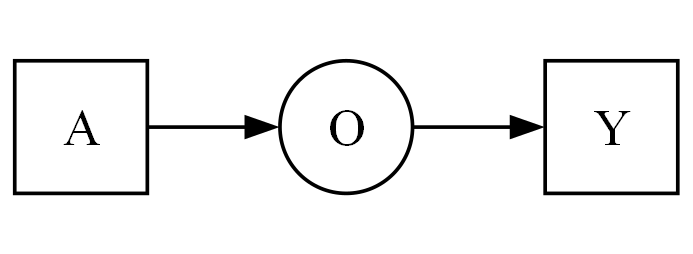
\includegraphics[width=2.5in,height=\textheight,keepaspectratio]{diagrams/fig-core-dag.png}

\caption{\label{fig-core-dag}\textbf{The shared identification
argument.} \(A\): age; \(O\): other unmeasured factors; \(Y\): the
vocabulary outcome. Conditioning on age identifies the total
age-associated change.}

\end{figure}%

\section{The outcome: a Beta-Binomial count}\label{sec-betabinomial}

We model each vocabulary outcome as a count bounded between \(0\) and
\(N_{\text{trials}}\) words, where \(N_{\text{trials}}\) is the number
of words on the reference checklist (a common 800-item reference
inventory throughout this report; see Section~\ref{sec-data} ). For
observation \(i\) at age \(x_i\) months we standardise age,

\[
z_i = \frac{x_i - \bar{x}}{s_x},
\]

so that a one-unit change in \(z\) corresponds to \(s_x\) months (this
scale differs by population and model --- see the relevant appendix).

A Binomial likelihood would assume exchangeable Bernoulli trials within
each observation and no unmodelled heterogeneity between children, so
its variance is fixed by its mean and it tends to \emph{underdisperse}
relative to real vocabulary data. To accommodate extra-binomial
variation we use a \textbf{Beta-Binomial} likelihood, in which the
per-observation success probability is itself Beta-distributed
(\citeproc{ref-gelmanBayesianDataAnalysis2013}{Gelman et al., 2013,
Section 17.2}; \citeproc{ref-qiaoBetaBinomialModelCount2025}{Qiao et
al., 2025}). With latent mean \(p_i = p(z_i)\) and concentration
\(\kappa_i > 0\),

\[
y_i \sim \mathrm{BetaBinomial}\!\left(N_{\text{trials}},\,\alpha_i,\,\beta_i\right),
\qquad
\alpha_i = p_i\,\kappa_i,
\qquad
\beta_i = (1-p_i)\,\kappa_i .
\]

Smaller \(\kappa_i\) implies greater dispersion (more between-child
heterogeneity at a given age); larger \(\kappa_i\) approaches the
Binomial. Observations are assumed conditionally independent given the
latent mean \(p(z)\), the dispersion \(\kappa(z)\), and the model
parameters.

\subsection{Age-varying dispersion}\label{sec-kappa}

Both experience and existing research indicate that variability in
vocabulary among children grows over time as children making more
progress diverge from those making less. We therefore let the
conditional distribution become more dispersed with age by modelling the
concentration as a decreasing function of age,

\[
\kappa(z) = \kappa_{\min} + \exp\!\left(a_\kappa + b_\kappa z\right),
\qquad b_\kappa < 0 .
\]

This encodes two assumptions. First, heterogeneity \textbf{increases}
with age: because \(b_\kappa < 0\), \(\exp(a_\kappa + b_\kappa z)\)
decreases, so \(\kappa(z)\) decreases and dispersion increases. Second,
the increase \textbf{levels off}: as \(z \to \infty\),
\(\kappa(z) \to \kappa_{\min}\), giving a later-age plateau in
dispersion. (Because the outcome is bounded, this does not require raw
count variance to increase monotonically at every age --- it allows
greater heterogeneity around the mean trajectory on the latent scale.)
We impose the monotone decline by setting
\(b_\kappa = -b_{\mathrm{mag}}\) with \(b_{\mathrm{mag}} > 0\).

\section{The mean trajectory}\label{sec-mean}

The latent mean trajectory is defined on the logit scale as a linear
trend plus a zero-mean Gaussian process (GP)
(\citeproc{ref-rasmussenGaussianProcessesMachine2008}{Rasmussen \&
Williams, 2008}; \citeproc{ref-schulzTutorialGaussianProcess2018}{Schulz
et al., 2018}):

\[
\begin{aligned}
f(z) &= \beta_0 + \beta_1 z + g(z), \qquad
p(z) = \sigma\!\left(f(z)\right) = \frac{1}{1 + e^{-f(z)}},\\
g(z) &= \eta\, g_{\mathrm{unit}}(z), \qquad
g_{\mathrm{unit}} \sim \mathcal{GP}\!\left(0,\, k(\cdot,\cdot)\right).
\end{aligned}
\]

The linear trend \(\beta_0 + \beta_1 z\) carries the expected population
trajectory; the GP \(g\) captures smooth deviations from it. We use a
zero mean function for \(g\) because any non-zero mean would be
confounded with the linear parameters --- so positive \(g(z)\) indicates
faster-than-expected growth and negative \(g(z)\) a slowdown or plateau,
and under the posterior \(g\) shrinks toward zero where data are sparse.

We use a unit-variance radial basis function (exponentiated-quadratic)
kernel,

\[
k(z,z') = \exp\!\left(-\frac{(z-z')^2}{2\ell^2}\right),
\qquad k(z,z) = 1,
\]

and factor out a separate amplitude \(\eta > 0\). This cleanly separates
two roles: the length-scale \(\ell\) governs how quickly deviations vary
with age (smoothness), while \(\eta\) governs how large they are. The
kernel is stationary (local smoothness is similar at, say, 36 and 72
months) and a universal approximator, which suits developmental
trajectories whose precise shape is unknown.

\subsection{Interpretable slope anchors}\label{sec-anchors}

Rather than placing weakly interpretable priors directly on \(\beta_0\)
and \(\beta_1\), we parameterise the linear trend through the expected
proportion of words at \textbf{two reference ages} \(x_a < x_b\). With
\(z_a = (x_a - \bar{x})/s_x\) and \(z_b = (x_b - \bar{x})/s_x\), and
priors placed on \(p_{x_a}\) and \(p_{x_b}\),

\[
\beta_1 = \frac{\operatorname{logit}(p_{x_b}) - \operatorname{logit}(p_{x_a})}{z_b - z_a},
\qquad
\beta_0 = \operatorname{logit}(p_{x_a}) - \beta_1 z_a .
\]

This gives an interpretable baseline on the logit scale while the GP
captures smooth departures. The reference ages and the priors on
\(p_{x_a}, p_{x_b}\) are \textbf{model-specific} (e.g.~24 and 84 months
for the Down syndrome models; 12 and 26 months for the typically
developing models) and are tabulated in each model's appendix.

\subsection{HSGP approximation}\label{sec-hsgp}

Exact GP inference requires an \(O(n^3)\) Cholesky factorisation. With
several hundred observations per model this is feasible but costly
inside MCMC, so we use the \textbf{Hilbert-space GP (HSGP)}
approximation
(\citeproc{ref-riutort-mayolPracticalHilbertSpace2022}{Riutort-Mayol et
al., 2022}; \citeproc{ref-solinHilbertSpaceMethods2020}{Solin \& Särkkä,
2020}), a finite basis-function representation that generates
\(g_{\mathrm{unit}}\) from a unit-variance kernel and then rescales by
\(\eta\). Approximation quality depends on the basis size \(m\)
(accuracy vs cost), the boundary factor \(c\) (must exceed the range of
observed \(z\)), and the length-scale \(\ell\) (shorter scales need more
basis functions). We select \(m\) and \(c\) following PyMC's
\texttt{approx\_hsgp\_hyperparams} recommendations for the specified
range of \(\ell\)
(\citeproc{ref-abril-plaPyMCModernComprehensive2023}{Abril-Pla et al.,
2023};
\citeproc{ref-riutort-mayolPracticalHilbertSpace2022}{Riutort-Mayol et
al., 2022}).

\section{Shared default priors}\label{sec-core-priors}

The following priors are held \textbf{constant across all models} (they
are the shared defaults in \texttt{definitions.py}). Model-specific
priors --- the slope anchors \(p_{x_a}, p_{x_b}\), and any
random-effect, GP-anchor or association settings --- are given in each
appendix as deltas from this table.

\begin{longtable}[]{@{}
  >{\raggedright\arraybackslash}p{(\linewidth - 4\tabcolsep) * \real{0.1250}}
  >{\raggedright\arraybackslash}p{(\linewidth - 4\tabcolsep) * \real{0.5000}}
  >{\raggedright\arraybackslash}p{(\linewidth - 4\tabcolsep) * \real{0.3750}}@{}}
\caption{Shared default prior distributions, identical across all
models.}\label{tbl-core-priors}\tabularnewline
\toprule\noalign{}
\begin{minipage}[b]{\linewidth}\raggedright
Parameter
\end{minipage} & \begin{minipage}[b]{\linewidth}\raggedright
Description
\end{minipage} & \begin{minipage}[b]{\linewidth}\raggedright
Prior
\end{minipage} \\
\midrule\noalign{}
\endfirsthead
\toprule\noalign{}
\begin{minipage}[b]{\linewidth}\raggedright
Parameter
\end{minipage} & \begin{minipage}[b]{\linewidth}\raggedright
Description
\end{minipage} & \begin{minipage}[b]{\linewidth}\raggedright
Prior
\end{minipage} \\
\midrule\noalign{}
\endhead
\bottomrule\noalign{}
\endlastfoot
\(\ell_\text{unit}\) & Unit length-scale, mapped linearly to 6--18
months & \(\mathrm{Beta}(3, 3)\) \\
\(\eta\) & GP amplitude (logit scale) &
\(\mathrm{HalfNormal}(\sigma = 0.4)\) \\
\(\kappa_{\min}\) & Minimum concentration (dispersion floor) &
\(\mathrm{LogNormal}(\mu = \log 5,\ \sigma = 0.6)\) \\
\(a_\kappa\) & Log-scale intercept of \(\kappa(z)\) &
\(\mathrm{Normal}(\mu = \log 8,\ \sigma = 1.0)\) \\
\(b_{\mathrm{mag}}\) & Magnitude of the \(\kappa\) decline rate
(\(b_\kappa = -b_{\mathrm{mag}}\)) &
\(\mathrm{HalfNormal}(\sigma = 0.3)\) \\
\end{longtable}

The length-scale is mapped from the unit interval onto a 6--18 month
range,
\(\ell = \ell_{\min} + (\ell_{\max} - \ell_{\min})\,\ell_\text{unit}\),
which favours changes over 6--18 month periods and offers better
sampling geometry than a direct prior on the positive reals. The
amplitude \(\eta\) is constant on the logit scale but, through the
logistic link, has its largest effect on counts near \(p \approx 0.5\)
(about 400 of 800 words) and least effect near the floor or ceiling ---
matching the expectation that there is least scope for variation when a
child is just starting out or near the checklist limit.

\section{Extension mechanisms}\label{extension-mechanisms}

The models differ only in which of the following mechanisms they switch
on. Each maps directly onto a field (or flag) in
\texttt{definitions.py}.

\subsection{Joint outcomes and production ratios}\label{sec-ratios}

The joint models estimate words \textbf{understood} and the conditional
probability that an understood word is also produced. With
\(p_U(a) = \sigma(f_U(a))\) for understanding, define the
\textbf{production ratio}

\[
q(a) = P(\text{speak} \mid \text{understood}) = \sigma(h(a)),
\qquad
p_S(a) = p_U(a)\,q(a),
\]

where \(f_U\) and \(h\) each have their own linear-trend-plus-GP
structure (Section~\ref{sec-mean}). Because \(q(a) \in (0,1)\), this
enforces \(p_S \le p_U\) by construction. The trivariate models add a
\textbf{sign ratio}

\[
r(a) = P(\text{sign} \mid \text{understood}) = \sigma(g_{\text{sign}}(a)),
\qquad
p_{\text{Sign}}(a) = p_U(a)\,r(a) .
\]

The signed mean \(g_{\text{sign}}\) is \textbf{intercept-only} (no age
slope) plus a GP: a free age slope extrapolates the signed ratio below
the data floor at young ages, so the GP alone carries the empirical
rise-then-fall hump. Each marginal outcome has its own Beta-Binomial
likelihood with its own age-varying dispersion
(Section~\ref{sec-betabinomial}, Section~\ref{sec-kappa}).

\subsection{Study and subject random
intercepts}\label{sec-randomeffects}

To separate the population age curves from differences in study
composition and from repeated measurements on the same child, we add
random intercepts on the logit-scale predictors at the observation
level. For a predictor \(f_\bullet \in \{f_U, h, g_{\text{sign}}\}\),

\[
f_\bullet(z_i) \;\to\; f_\bullet(z_i) + \delta^{\text{study}}_{\bullet,\,s(i)} + \delta^{\text{subj}}_{\bullet,\,j(i)},
\qquad
\delta_\bullet \sim \mathrm{Normal}(0, \tau_\bullet),\ \ \tau_\bullet \sim \mathrm{HalfNormal}(0.5),
\]

implemented non-centred, where \(s(i)\) and \(j(i)\) index the study and
subject of observation \(i\). Study intercepts absorb
between-lab/between-study level differences; subject intercepts stop
within-child repeated measurements being treated as independent.
\textbf{The reported population curves set every random effect to zero},
so their interpretation is unchanged. Tiny studies can be trimmed before
fitting (\texttt{min\_study\_observations}) to avoid near-unidentified
intercepts.

\subsection{Gaussian-process anchoring}\label{sec-gpanchor}

Once a random intercept and the linear/intercept term and the GP can
each carry the global level, that level becomes redundant and sampling
geometry degrades (a GP↔intercept ridge). We remove the redundancy by
constraining each GP to pass through zero at a reference age
\(a_{\text{ref}}\) \textbf{for every posterior draw},

\[
\tilde{g}(z) = \eta\left(g_{\mathrm{unit}}(z) - g_{\mathrm{unit}}(z_{\text{ref}})\right),
\]

so the level is owned solely by the linear/intercept term and the random
effects, while the GP carries only the \emph{shape} of departures around
\(a_{\text{ref}}\). The reference age \(a_{\text{ref}}\)
(\texttt{gp\_anchor\_age\_months}) is model-specific.

\subsection{Within-understood sign--speech
association}\label{sec-association}

For each understood word a child may sign it, speak it, both, or
neither. The trivariate marginals \(r\) and \(q\)
(Section~\ref{sec-ratios}) leave the \textbf{overlap} unidentified; the
joint model adds a single scalar \textbf{Plackett odds ratio} \(\psi\)
linking sign and speech within understood words via the copula
\(C(r, q; \psi)\):

\[
\pi_{\text{both}} = C(r, q; \psi),\quad
\pi_{\text{sign-only}} = r - \pi_{\text{both}},\quad
\pi_{\text{speak-only}} = q - \pi_{\text{both}},\quad
\pi_{\text{neither}} = 1 - r - q + \pi_{\text{both}} .
\]

\(\psi = 1\) is independence (\(\pi_{\text{both}} = r\,q\));
\(\psi > 1\) means a word is signed and spoken together more often than
independence predicts. The four cells are fitted with a
Dirichlet-Multinomial likelihood, identified from the four-cell
cross-tabulation (the uk\_02 data; see Section~\ref{sec-data} ). The
association yields a \textbf{data-identified total expressive
vocabulary}

\[
p_{\text{any}}(a) = p_U(a)\left(r(a) + q(a) - \pi_{\text{both}}(a)\right),
\]

which sits below an independence-based upper bound whenever
\(\psi > 1\).

\begin{tcolorbox}[enhanced jigsaw, arc=.35mm, bottomrule=.15mm, bottomtitle=1mm, breakable, colback=white, colbacktitle=quarto-callout-important-color!10!white, colframe=quarto-callout-important-color-frame, coltitle=black, left=2mm, leftrule=.75mm, opacityback=0, opacitybacktitle=0.6, rightrule=.15mm, title=\textcolor{quarto-callout-important-color}{\faExclamation}\hspace{0.5em}{Important}, titlerule=0mm, toprule=.15mm, toptitle=1mm]

\(\psi\) is a \textbf{single scalar}, identified from a small four-cell
cross-tab, and is treated as \textbf{descriptive / exploratory}
throughout this report. See \textbf{?@sec-findings-signing} for its
scope and caveats.

\end{tcolorbox}

\chapter{Bayesian workflow and model
validation}\label{bayesian-workflow-and-model-validation}

\emph{This chapter describes the iterative Bayesian workflow used to
develop, fit and validate the models: the fitting pipeline and sampling
configurations, the validation checks every model is held to (prior
predictive, convergence diagnostics, posterior predictive), and the
formal basis on which one model is said to supersede another ---
tabulated out-of-sample model comparison together with identified
structural issues.}

\hfill\break

\begin{tcolorbox}[enhanced jigsaw, arc=.35mm, bottomrule=.15mm, bottomtitle=1mm, breakable, colback=white, colbacktitle=quarto-callout-note-color!10!white, colframe=quarto-callout-note-color-frame, coltitle=black, left=2mm, leftrule=.75mm, opacityback=0, opacitybacktitle=0.6, rightrule=.15mm, title=\textcolor{quarto-callout-note-color}{\faInfo}\hspace{0.5em}{Note}, titlerule=0mm, toprule=.15mm, toptitle=1mm]

Drafted by an LLM-based AI tool (Claude Code/Opus 4.8).

\end{tcolorbox}

\section{The iterative workflow}\label{the-iterative-workflow}

\textbf{TODO}: summarise the Bayesian workflow
(\citeproc{ref-gelmanBayesianWorkflow2020}{Gelman, Vehtari, et al.,
2020}) as applied here --- build simple, check, extend, compare --- and
forward-reference the two development lineages
(\textbf{?@sec-lineage-ds}, \textbf{?@sec-lineage-signing}) that
instantiate it.

\section{Fitting pipeline and sampling
configurations}\label{fitting-pipeline-and-sampling-configurations}

\textbf{TODO}: PyMC with the nutpie sampler; the \texttt{fit(config)}
pipeline stages (data prep → build → prior predictive → MCMC →
diagnostics → posterior predictive → summary → plots → report); the
\texttt{dev} / \texttt{test} / \texttt{rep} sampling configurations and
which results in this report are \texttt{rep}-quality. (Full
reproduction in Appendix D.)

\section{Validation checks}\label{validation-checks}

Every model in this report is held to the same checks; the per-model
evidence is in Appendix B.

\subsection{Prior predictive checks}\label{prior-predictive-checks}

\textbf{TODO}: what we require of the priors before fitting (plausible
age--vocabulary curves: low counts young, smooth change, widening spread
with age, no mass on impossible values).

\subsection{Convergence diagnostics}\label{convergence-diagnostics}

Every reported fit must clear a single, explicit convergence gate before
any estimate is read from it: no divergent transitions, a potential
scale reduction factor \(\hat{R} \le 1.01\) on all parameters, bulk and
tail effective sample size (ESS) \(\ge 400\), and an energy Bayesian
fraction of missing information (BFMI) \(\ge 0.3\) on every chain. These
thresholds are applied uniformly across all models, and each model's
appendix entry carries a generated pass/fail banner that records them
against the achieved values (\textbf{?@sec-appendix-b1}). The
\texttt{rep}-quality fits reported here clear the gate; where a
development-configuration fit does not --- short chains routinely miss
the ESS target --- its estimates are treated as provisional until
refitted at reporting quality.

\subsection{Posterior predictive
checks}\label{posterior-predictive-checks}

\textbf{TODO}: how fitted models are checked against observed counts
(PMF/CDF overlays, count distributions by age, the four-cell PPC for the
signing model).

\subsection{Reporting estimates: lead with the
interval}\label{reporting-estimates-lead-with-the-interval}

Several estimands in this report rest on modest samples --- most acutely
the sign--speech association \(\psi\), identified from roughly 34
children. At that precision a point estimate selected because it looks
``significant'' (for example, because its interval excludes a reference
value) is on average inflated in magnitude, and at low power can even
take the wrong sign --- the Type-M and Type-S errors that follow from
selecting on a noisy estimate (the ``winner's curse''). We therefore
lead with the credible interval and the strength of evidence for a named
claim, and treat the point estimate as the least informative summary
rather than the headline.

\section{Model comparison and what ``supersedes''
means}\label{sec-supersedes}

A later model is said to \textbf{supersede} an earlier one only on two
combined grounds, reported together:

\begin{enumerate}
\def\labelenumi{\arabic{enumi}.}
\tightlist
\item
  \textbf{Tabulated out-of-sample comparison} --- LOO / expected log
  pointwise predictive density (ELPD), reported as a comparison table
  with standard errors of the difference, so the improvement is
  quantified rather than asserted.
\item
  \textbf{Identified structural issue} --- a concrete, named modelling
  problem in the earlier model that the later one resolves (e.g.~study
  composition confounding a population curve; a GP↔intercept
  identifiability ridge; an independence assumption that is not
  data-identified).
\end{enumerate}

\textbf{TODO}: present the master model-comparison table here (or
cross-reference the per-lineage tables in Part III), and define the
status taxonomy used throughout --- \emph{model of record},
\emph{development step}, \emph{TD reference}, \emph{superseded} ---
enforced as a rule that superseded models never source a number in the
findings (see Appendix A for the full register).

\section{Provenance and
reproducibility}\label{provenance-and-reproducibility}

\textbf{TODO}: the per-render provenance stamp (model id + git revision
+ sampling configuration, generated rather than hand-written) carried by
every result chapter; \texttt{freeze:\ true} for pinned editions; the
relationship to the live per-fit dashboards in
\texttt{docs/models/vgNN}. (Full detail in Appendix D.)

\part{Results}

\chapter{Words understood and spoken}\label{words-understood-and-spoken}

{[}TODO{]}

\hfill\break

{[}TODO{]}

\chapter{Words signed and total expressive
vocabulary}\label{words-signed-and-total-expressive-vocabulary}

\emph{TODO}

\hfill\break

{[}TODO{]}

\part{Discussion}

\chapter{Discussion}\label{discussion-1}

Summary --- \emph{TODO}

\hfill\break

TODO

\part{Appendices}

\chapter{Appendix B --- Model
specifications}\label{appendix-b-model-specifications}

TODO

\hfill\break

\chapter{Appendix C --- Reference
tables}\label{appendix-c-reference-tables}

\emph{TODO}

\hfill\break

TODO

\chapter{Appendix E --- Use of AI}\label{appendix-e-use-of-ai}

\emph{How LLM-based AI tools were used in preparing this report and the
safeguards applied to generated content.}

\hfill\break

\begin{tcolorbox}[enhanced jigsaw, arc=.35mm, bottomrule=.15mm, bottomtitle=1mm, breakable, colback=white, colbacktitle=quarto-callout-note-color!10!white, colframe=quarto-callout-note-color-frame, coltitle=black, left=2mm, leftrule=.75mm, opacityback=0, opacitybacktitle=0.6, rightrule=.15mm, title=\textcolor{quarto-callout-note-color}{\faInfo}\hspace{0.5em}{Note}, titlerule=0mm, toprule=.15mm, toptitle=1mm]

Drafted by an LLM-based AI tool (Codex/GPT-5).

\end{tcolorbox}

LLM-based AI tools may be used in this project as drafting, coding,
editing and review assistants. AI-assisted document sections are
labelled near the top of the relevant Markdown or Quarto file, following
the repository convention.

The human authors remain responsible for the study design, data
handling, model specification, interpretation, verification and final
wording. AI-assisted changes must be reviewed against the source data,
fitted model output, cited literature and repository checks before
publication.

\chapter*{References}\label{references}
\addcontentsline{toc}{chapter}{References}

\markboth{References}{References}

\protect\phantomsection\label{refs}
\begin{CSLReferences}{1}{0}
\bibitem[\citeproctext]{ref-abbedutoLanguageDevelopmentSyndrome2020}
Abbeduto, L., Arias-Trejo, N., Thurman, A. J., Ramos-Sanchez, J., \& Del
Hoyo Soriano, L. (2020). Language {Development} in {Down Syndrome}. In
L. Abbeduto, N. Arias-Trejo, A. J. Thurman, J. Ramos-Sanchez, \& L. Del
Hoyo Soriano, \emph{The {Oxford Handbook} of {Down Syndrome} and
{Development}}. Oxford University Press.
\url{https://doi.org/10.1093/oxfordhb/9780190645441.013.18}

\bibitem[\citeproctext]{ref-abril-plaPyMCModernComprehensive2023}
Abril-Pla, O., Andreani, V., Carroll, C., Dong, L., Fonnesbeck, C. J.,
Kochurov, M., Kumar, R., Lao, J., Luhmann, C. C., Martin, O. A.,
Osthege, M., Vieira, R., Wiecki, T., \& Zinkov, R. (2023). {PyMC}: A
modern, and comprehensive probabilistic programming framework in
{Python}. \emph{PeerJ Computer Science}, \emph{9}, e1516.
\url{https://doi.org/10.7717/peerj-cs.1516}

\bibitem[\citeproctext]{ref-bayesLIIEssaySolving1763}
Bayes, T., \& Price, R. (1763). {LII}. {An} essay towards solving a
problem in the doctrine of chances. {By} the late {Rev}. {Mr}. {Bayes},
{F}. {R}. {S}. Communicated by {Mr}. {Price}, in a letter to {John
Canton}, {A}. {M}. {F}. {R}. {S}. \emph{Philosophical Transactions of
the Royal Society of London}, \emph{53}, 370--418.
\url{https://doi.org/10.1098/rstl.1763.0053}

\bibitem[\citeproctext]{ref-berglundParentalReportsSpoken2001}
Berglund, E., Eriksson, M., \& Johansson, I. (2001). Parental {Reports}
of {Spoken Language Skills} in {Children With Down Syndrome}.
\emph{Journal of Speech, Language, and Hearing Research}, \emph{44}(1),
179--191. \url{https://doi.org/10.1044/1092-4388(2001/016)}

\bibitem[\citeproctext]{ref-bernardoBayesianStatistics2025}
Bernardo, J. M. (2025). Bayesian {Statistics}. In \emph{International
{Encyclopedia} of {Statistical Science}} (pp. 199--233). Springer,
Berlin, Heidelberg. \url{https://doi.org/10.1007/978-3-662-69359-9_59}

\bibitem[\citeproctext]{ref-bonBeingBayesian2020s2023}
Bon, J. J., Bretherton, A., Buchhorn, K., Cramb, S., Drovandi, C.,
Hassan, C., Jenner, A. L., Mayfield, H. J., McGree, J. M., Mengersen,
K., Price, A., Salomone, R., Santos-Fernandez, E., Vercelloni, J., \&
Wang, X. (2023). Being {Bayesian} in the 2020s: Opportunities and
challenges in the practice of modern applied {Bayesian} statistics.
\emph{Philosophical Transactions of the Royal Society A: Mathematical,
Physical and Engineering Sciences}, \emph{381}(2247), 20220156.
\url{https://doi.org/10.1098/rsta.2022.0156}

\bibitem[\citeproctext]{ref-chanStatisticalModelingComputation2025}
Chan, J. C. C., \& Kroese, D. P. (2025). \emph{Statistical {Modeling}
and {Computation}}. Springer US.
\url{https://doi.org/10.1007/978-1-0716-4132-3}

\bibitem[\citeproctext]{ref-coxPrinciplesStatisticalInference2006}
Cox, D. R. (2006). \emph{Principles of statistical inference}. Cambridge
university press.

\bibitem[\citeproctext]{ref-cristescuShapeResearchChange2024}
Cristescu, L., Scerif, G., Pellicano, L., Van Herwegen, J., \& Farran,
E. K. (2024, June 4). \emph{Shape {Research}, {Change Lives}: {Setting}
priorities in genetic syndrome research}.
\url{https://doi.org/10.31234/osf.io/whbfp}

\bibitem[\citeproctext]{ref-dsouzaExplainingComprehensionProduction2026}
D'Souza, D., D'Souza, H., Mayor, J., \& Tovar, Á. E. (2026). Explaining
the {Comprehension}--{Production Vocabulary Gap Through Neural Networks}
and {Cross-Syndrome Evidence}: {Insights From Williams Syndrome}.
\emph{Developmental Science}, \emph{29}(2), e70115.
\url{https://doi.org/10.1111/desc.70115}

\bibitem[\citeproctext]{ref-deckersPredictorsReceptiveExpressive2019}
Deckers, S. R. J. M., Van Zaalen, Y., Van Balkom, H., \& Verhoeven, L.
(2019). Predictors of receptive and expressive vocabulary development in
children with {Down} syndrome. \emph{International Journal of
Speech-Language Pathology}, \emph{21}(1), 10--22.
\url{https://doi.org/10.1080/17549507.2017.1363290}

\bibitem[\citeproctext]{ref-farrellComputationalModelingCognition2018}
Farrell, S., \& Lewandowsky, S. (2018). \emph{Computational {Modeling}
of {Cognition} and {Behavior}}. Cambridge University Press.
\url{https://doi.org/10.1017/CBO9781316272503}

\bibitem[\citeproctext]{ref-frankWordbankOpenRepository2017}
Frank, M. C., Braginsky, M., Yurovsky, D., \& Marchman, V. A. (2017).
Wordbank: An open repository for developmental vocabulary data.
\emph{Journal of Child Language}, \emph{44}(3), 677--694.
\url{https://doi.org/10.1017/S0305000916000209}

\bibitem[\citeproctext]{ref-galeoteAcquisitionProductiveVocabulary2008}
Galeote, M., Soto, P., Checa, E., Gómez, A., \& Lamela, E. (2008). The
acquisition of productive vocabulary in {Spanish} children with {Down}
syndrome. \emph{Journal of Intellectual \& Developmental Disability},
\emph{33}(4), 292--302. \url{https://doi.org/10.1080/13668250802441870}

\bibitem[\citeproctext]{ref-gelmanBayesianDataAnalysis2013}
Gelman, A., Carlin, J. B., Stern, H. S., Dunson, D. B., Vehtari, A., \&
Rubin, D. B. (2013). \emph{Bayesian {Data Analysis}} (3rd ed.). {Chapman
and Hall/CRC}. \url{https://doi.org/10.1201/b16018}

\bibitem[\citeproctext]{ref-gelmanRegressionOtherStories2020}
Gelman, A., Hill, J., \& Vehtari, A. (2020). \emph{Regression and {Other
Stories}}. Cambridge University Press.
\url{https://doi.org/10.1017/9781139161879}

\bibitem[\citeproctext]{ref-gelmanBayesianWorkflow2020}
Gelman, A., Vehtari, A., Simpson, D., Margossian, C. C., Carpenter, B.,
Yao, Y., Kennedy, L., Gabry, J., Bürkner, P.-C., \& Modrák, M. (2020,
November 3). \emph{Bayesian {Workflow}}.
\url{https://doi.org/10.48550/arXiv.2011.01808}

\bibitem[\citeproctext]{ref-gillBayesianSocialScience2024}
Gill, J., \& Bao, L. (2024). \emph{Bayesian {Social Science Statistics}:
{From} the {Very Beginning}} (1st ed.). Cambridge University Press.
\url{https://doi.org/10.1017/9781009341189}

\bibitem[\citeproctext]{ref-gillBayesianModelingInference2020}
Gill, J., \& Heuberger, S. (2020). Bayesian {Modeling} and {Inference}:
{A Postmodern Perspective}. In L. Curini \& R. Franzese, \emph{The {SAGE
Handbook} of {Research Methods} in {Political Science} and
{International Relations}} (pp. 961--984). SAGE Publications Ltd.
\url{https://doi.org/10.4135/9781526486387.n53}

\bibitem[\citeproctext]{ref-hastingsMonteCarloSampling1970}
Hastings, W. K. (1970). Monte {Carlo} sampling methods using {Markov}
chains and their applications. \emph{Biometrika}, \emph{57}(1), 97--109.
\url{https://doi.org/10.1093/biomet/57.1.97}

\bibitem[\citeproctext]{ref-hoekstraRobustMisinterpretationConfidence2014}
Hoekstra, R., Morey, R. D., Rouder, J. N., \& Wagenmakers, E.-J. (2014).
Robust misinterpretation of confidence intervals. \emph{Psychonomic
Bulletin \& Review}, \emph{21}(5), 1157--1164.
\url{https://doi.org/10.3758/s13423-013-0572-3}

\bibitem[\citeproctext]{ref-hoffmanNoUTurnSamplerAdaptively2014}
Hoffman, M. D., \& Gelman, A. (2014). The {No-U-Turn Sampler}:
{Adaptively Setting Path Lengths} in {Hamiltonian Monte Carlo}.
\emph{Journal of Machine Learning Research}, \emph{15}(47), 1593--1623.
\url{http://jmlr.org/papers/v15/hoffman14a.html}

\bibitem[\citeproctext]{ref-hulmeGrowthReadingSkills2012}
Hulme, C., Goetz, K., Brigstocke, S., Nash, H. M., Lerv??g, A., \&
Snowling, M. J. (2012). The growth of reading skills in children with
{Down Syndrome}. \emph{Developmental Science}, \emph{15}(3), 320--329.
\url{https://doi.org/10.1111/j.1467-7687.2011.01129.x}

\bibitem[\citeproctext]{ref-kaat-vandenosExpressiveVocabularyDevelopment2017}
Kaat-van Den Os, D. T., Volman, C., Jongmans, M., \& Lauteslager, P.
(2017). Expressive {Vocabulary Development} in {Children With Down
Syndrome}: {A Longitudinal Study}: {Vocabulary Growth} and {Profiles}.
\emph{Journal of Policy and Practice in Intellectual Disabilities},
\emph{14}(4), 311--318. \url{https://doi.org/10.1111/jppi.12212}

\bibitem[\citeproctext]{ref-kruschkeBayesianAnalysisReporting2021}
Kruschke, J. K. (2021). Bayesian {Analysis Reporting Guidelines}.
\emph{Nature Human Behaviour}, \emph{5}(10), 1282--1291.
\url{https://doi.org/10.1038/s41562-021-01177-7}

\bibitem[\citeproctext]{ref-LaplaceMemoireProbabilite}
LaPlace, P. S. (1774). Mémoire sur la {Probabilité} des {Causes} par les
évènemens. \emph{Mémoires de Mathematique Et de Physique, Presentés à
l'Académie Royale Des Sciences, Par Divers Savans \& Lus Dans Ses
Assemblées, Tome Sixième}, 621--656.
\url{https://www.scirp.org/reference/referencespapers?referenceid=1055232}

\bibitem[\citeproctext]{ref-laplaceEssaiPhilosophiqueProbabilites1814}
LaPlace, P. S. (1814). \emph{Essai philosophique sur les probabilités}.
\url{https://eudml.org/doc/203193}

\bibitem[\citeproctext]{ref-laplaceTheorieAnalytiqueProbabilites1820}
LaPlace, P. S. (1820). \emph{Théorie analytique des probabilités}.
\url{https://eudml.org/doc/203444}

\bibitem[\citeproctext]{ref-martingklusekjestigarribiabjLanguageCharacteristicsIndividuals2009}
Martin, K., G. (2009). Language {Characteristics} of {Individuals With
Down Syndrome}. \emph{Topics in Language Disorders}, 112--132.

\bibitem[\citeproctext]{ref-mcelreathStatisticalRethinkingBayesian2020}
McElreath, R. (2020). \emph{Statistical {Rethinking}: {A Bayesian
Course} with {Examples} in {R} and {STAN}} (2nd ed.). {Chapman and
Hall/CRC}. \url{https://doi.org/10.1201/9780429029608}

\bibitem[\citeproctext]{ref-metropolisEquationStateCalculations1953}
Metropolis, N., Rosenbluth, A. W., Rosenbluth, M. N., Teller, A. H., \&
Teller, E. (1953). Equation of {State Calculations} by {Fast Computing
Machines}. \emph{The Journal of Chemical Physics}, \emph{21}(6),
1087--1092. \url{https://doi.org/10.1063/1.1699114}

\bibitem[\citeproctext]{ref-moreyFallacyPlacingConfidence2016}
Morey, R. D., Hoekstra, R., Rouder, J. N., Lee, M. D., \& Wagenmakers,
E.-J. (2016). The fallacy of placing confidence in confidence intervals.
\emph{Psychonomic Bulletin \& Review}, \emph{23}(1), 103--123.
\url{https://doi.org/10.3758/s13423-015-0947-8}

\bibitem[\citeproctext]{ref-naessLanguageVerbalShortterm2011}
Næss, K.-A. B., Lyster, S.-A. H., Hulme, C., \& Melby-Lervåg, M. (2011).
Language and verbal short-term memory skills in children with {Down}
syndrome: {A} meta-analytic review. \emph{Research in Developmental
Disabilities}, \emph{32}(6), 2225--2234.
\url{https://doi.org/10.1016/j.ridd.2011.05.014}

\bibitem[\citeproctext]{ref-naessReadingSkillsChildren2012}
Næss, K.-A. B., Melby-Lervåg, M., Hulme, C., \& Lyster, S.-A. H. (2012).
Reading skills in children with {Down} syndrome: A meta-analytic review.
\emph{Research in Developmental Disabilities}, \emph{33}(2), 737--747.
\url{https://doi.org/10.1016/j.ridd.2011.09.019}

\bibitem[\citeproctext]{ref-naessDifferencesSimilaritiesPredictors2021}
Næss, K.-A. B., Ostad, J., \& Nygaard, E. (2021). Differences and
{Similarities} in {Predictors} of {Expressive Vocabulary Development}
between {Children} with {Down Syndrome} and {Young Typically Developing
Children}. \emph{Brain Sciences}, \emph{11}(3), 312.
\url{https://doi.org/10.3390/brainsci11030312}

\bibitem[\citeproctext]{ref-oliverLanguageDevelopmentChildren1994}
Oliver, B., \& Buckley, S. (1994). The language development of children
with {Down}'s syndrome: {First} words to two-word phrases. \emph{Down
Syndrome Research and Practice}, \emph{2}(2), 71--75.
\url{https://doi.org/10.3104/reports.33}

\bibitem[\citeproctext]{ref-pfadtMethodologicalMetamorphosisRapid2025}
Pfadt, J. M., Bartoš, F., Godmann, H. R., Waaijers, M., Groot, L., Heo,
I., Mensink, L., Nak, J., De Ruiter, J. P., Sarafoglou, A., Siepe, B.
S., Arena, G., Mr., Akrong, E., Aust, F., van den Bergh, D., Brenner,
W., Doekemeijer, R. A., Donzallaz, M. C., van Doorn, J., \ldots{}
Wagenmakers, E.-J. (2025, October 30). \emph{A {Methodological
Metamorphosis}: {The Rapid Rise} of {Bayesian Inference} and {Open
Science Practices} in {Psychology}} (ck3js\_v1).
\url{https://doi.org/10.31234/osf.io/ck3js_v1} (Pre-published)

\bibitem[\citeproctext]{ref-qiaoBetaBinomialModelCount2025}
Qiao, X., Kamata, A., Kara, Y., Potgieter, C., \& Nese, J. F. T. (2025).
Beta-{Binomial Model} for {Count Data}: {An Application} in {Estimating
Model-Based Oral Reading Fluency}. \emph{Educational and Psychological
Measurement}, \emph{85}(6), 1200--1224.
\url{https://doi.org/10.1177/00131644251335914}

\bibitem[\citeproctext]{ref-rasmussenGaussianProcessesMachine2008}
Rasmussen, C. E., \& Williams, C. K. I. (2008). \emph{Gaussian processes
for machine learning} (3. print). MIT Press.
\url{https://doi.org/10.7551/mitpress/3206.001.0001}

\bibitem[\citeproctext]{ref-riutort-mayolPracticalHilbertSpace2022}
Riutort-Mayol, G., Bürkner, P.-C., Andersen, M. R., Solin, A., \&
Vehtari, A. (2022). Practical {Hilbert} space approximate {Bayesian
Gaussian} processes for probabilistic programming. \emph{Statistics and
Computing}, \emph{33}(1), 17.
\url{https://doi.org/10.1007/s11222-022-10167-2}

\bibitem[\citeproctext]{ref-schubertImprovingStatisticalReporting2025}
Schubert, A.-L., Steinhilber, M., Kang, H., \& Quintana, D. S. (2025).
Improving statistical reporting in psychology. \emph{Communications
Psychology}, \emph{3}(1), 156.
\url{https://doi.org/10.1038/s44271-025-00356-w}

\bibitem[\citeproctext]{ref-schulzTutorialGaussianProcess2018}
Schulz, E., Speekenbrink, M., \& Krause, A. (2018). A tutorial on
{Gaussian} process regression: {Modelling}, exploring, and exploiting
functions. \emph{Journal of Mathematical Psychology}, \emph{85}, 1--16.
\url{https://doi.org/10.1016/j.jmp.2018.03.001}

\bibitem[\citeproctext]{ref-solinHilbertSpaceMethods2020}
Solin, A., \& Särkkä, S. (2020). Hilbert space methods for reduced-rank
{Gaussian} process regression. \emph{Statistics and Computing},
\emph{30}(2), 419--446. \url{https://doi.org/10.1007/s11222-019-09886-w}

\bibitem[\citeproctext]{ref-spanosProbabilityTheoryStatistical2019}
Spanos, A. (2019). \emph{Probability {Theory} and {Statistical
Inference}: {Empirical Modeling} with {Observational Data}} (2nd ed.).
Cambridge University Press. \url{https://doi.org/10.1017/9781316882825}

\bibitem[\citeproctext]{ref-standevelopmentteamStanLanguageReference2026}
Stan Development Team. (2026). \emph{Stan {Language Reference Manual}
2.38}. \url{https://mc-stan.org/docs/reference-manual/}

\bibitem[\citeproctext]{ref-vanoijenBayesianCompendium2024}
Van Oijen, M. (2024). \emph{Bayesian {Compendium}}. Springer
International Publishing.
\url{https://doi.org/10.1007/978-3-031-66085-6}

\bibitem[\citeproctext]{ref-wagenmakersBayesianFrequentistInference2008}
Wagenmakers, E.-J., Lee, M., Lodewyckx, T., \& Iverson, G. J. (2008).
Bayesian {Versus Frequentist Inference}. In H. Hoijtink, I. Klugkist, \&
P. A. Boelen (Eds.), \emph{Bayesian {Evaluation} of {Informative
Hypotheses}} (pp. 181--207). Springer.
\url{https://doi.org/10.1007/978-0-387-09612-4_9}

\bibitem[\citeproctext]{ref-wagenmakersBayesianInferencePsychology2018}
Wagenmakers, E.-J., Marsman, M., Jamil, T., Ly, A., Verhagen, J., Love,
J., Selker, R., Gronau, Q. F., Šmíra, M., Epskamp, S., Matzke, D.,
Rouder, J. N., \& Morey, R. D. (2018). Bayesian inference for
psychology. {Part I}: {Theoretical} advantages and practical
ramifications. \emph{Psychonomic Bulletin \& Review}, \emph{25}(1),
35--57. \url{https://doi.org/10.3758/s13423-017-1343-3}

\bibitem[\citeproctext]{ref-wakefieldBayesianFrequentistRegression2013}
Wakefield, J. (2013). \emph{Bayesian and {Frequentist Regression
Methods}}. Springer. \url{https://doi.org/10.1007/978-1-4419-0925-1}

\bibitem[\citeproctext]{ref-zampiniVocabularyDevelopmentChildren2013}
Zampini, L., \& D'Odorico, L. (2013). Vocabulary development in children
with {Down} syndrome: Longitudinal and cross-sectional data.
\emph{Journal of Intellectual \& Developmental Disability}, \emph{38},
310--317. \url{https://doi.org/10.3109/13668250.2013.828833}

\end{CSLReferences}




\end{document}
